\par{...\ref{tilingResults}}

\begin{figure}[!h]
    \centering
    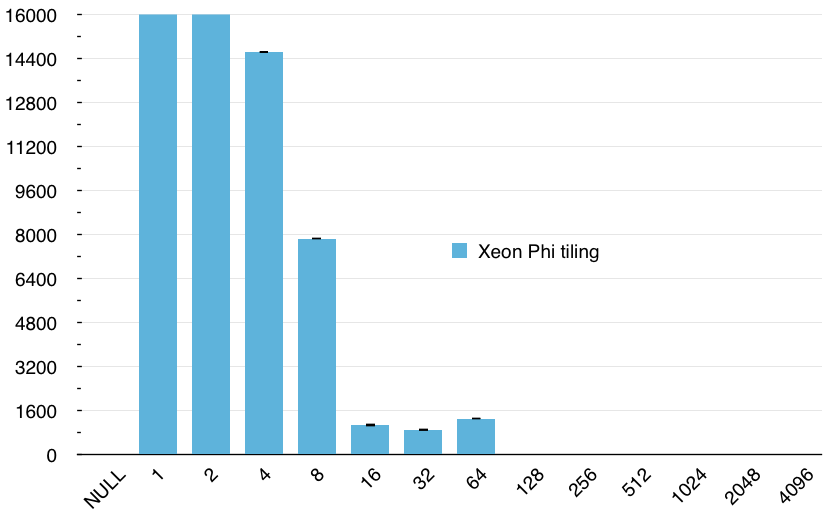
\includegraphics[width=0.4\textwidth]{figures/phiTiling.png}
    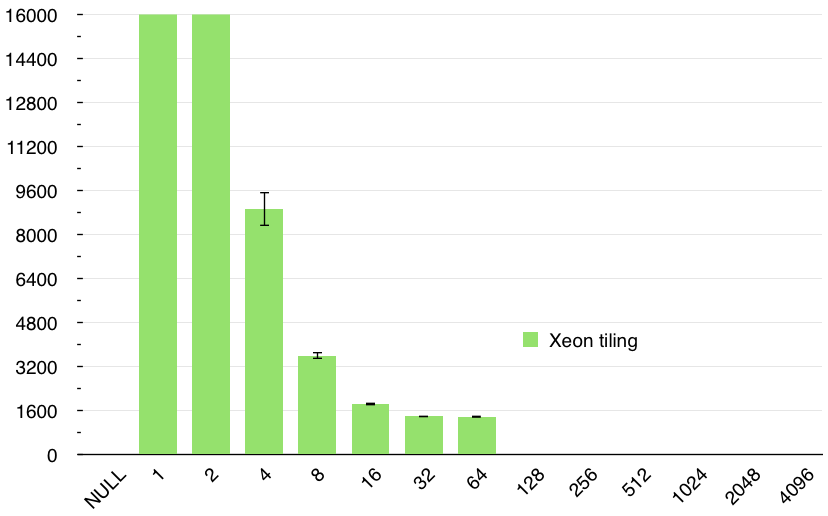
\includegraphics[width=0.4\textwidth]{figures/xeonTiling.png}
    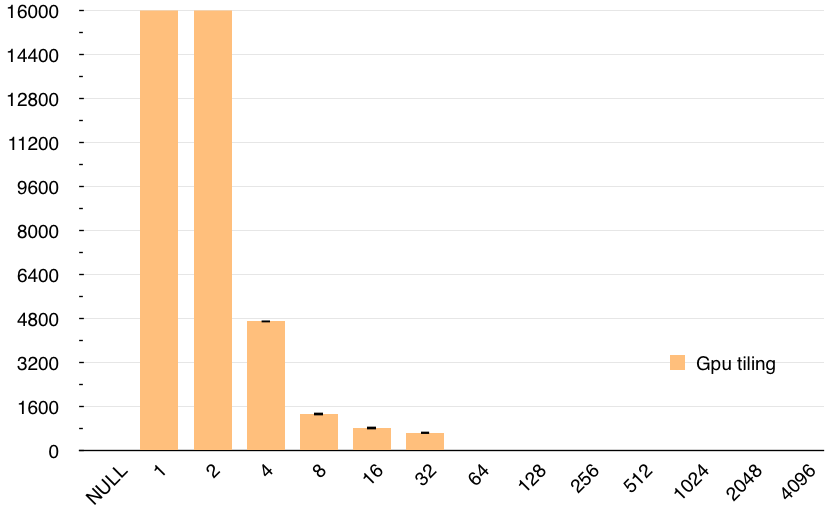
\includegraphics[width=0.4\textwidth]{figures/gpuTiling.png}
    \caption{Results for tiling.}
    \label{tilingResults}
\end{figure}

\par{Listing \ref{tiling} shows the algorithm.}

\par{loading a tile in to local memory, execution in phases, plus barrier synchronization }

\par{execution will be divided in phases, every phase data accesses will be in a tile of A and a tile of B}
\par{work items in a work group participate in loading a tile}
\par{Now Im passing the kernel 2 more arguments than naive implementation, for storing in local memory tilings of A and B}
\par{first barrier waits for all the work items to load the data into local memory}
\par{every work-time maintains running variable in registers}
\par{improvement of number of floating point operations per load instructions, and this improves as the block size increase}

\subsubsection{Summary Matrix Matrix Multiplication}

\par{Figure \ref{gpu}, \ref{phi} and \ref{xeon} shows the summary of the results of all the changes in the kernels for matrix
    matrix multiplication.}

\begin{figure}[!h]
    \centering
    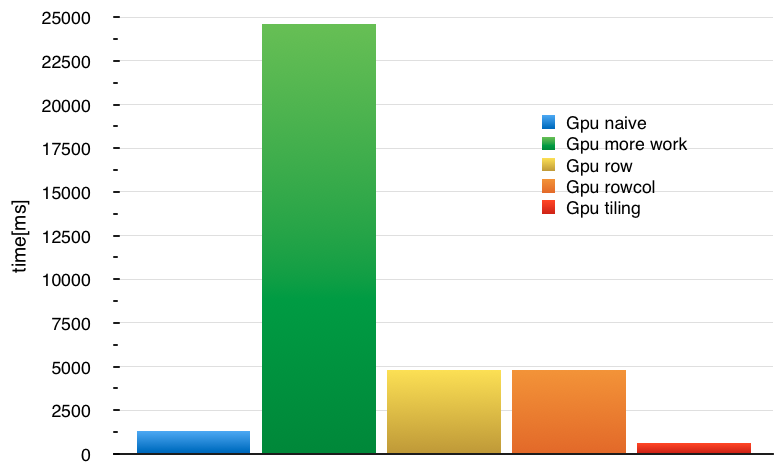
\includegraphics[width=0.4\textwidth]{figures/gpu.png}
    \caption{Matrix Matrix multiplication optimisations GPU.}
    \label{gpu}
\end{figure}

\begin{figure}[!h]
    \centering
    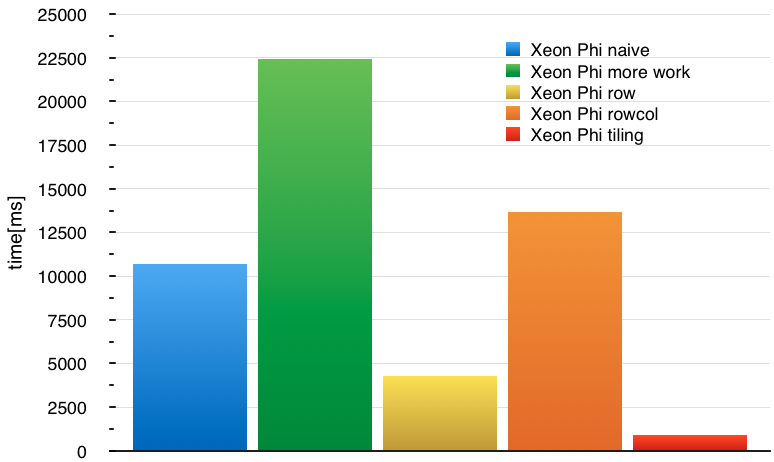
\includegraphics[width=0.4\textwidth]{figures/phi.png}
    \caption{Matrix Matrix multiplication optimisations Xeon Phi.}
    \label{phi}
\end{figure}

\begin{figure}[!h]
    \centering
    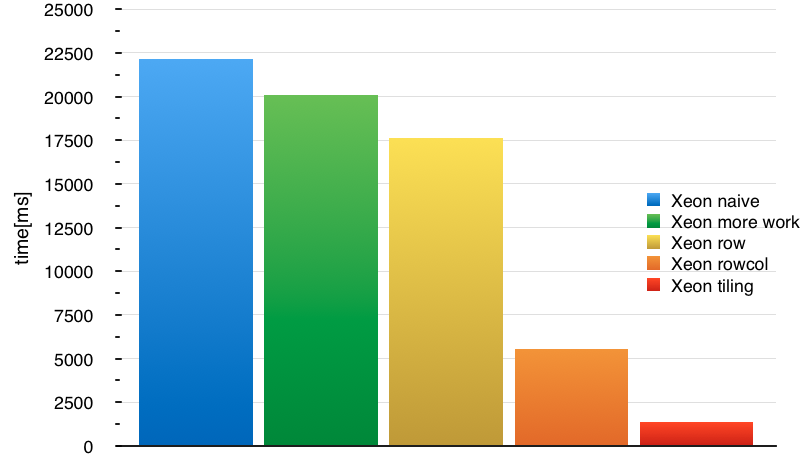
\includegraphics[width=0.4\textwidth]{figures/xeon.png}
    \caption{Matrix Matrix multiplication optimisations Xeon.}
    \label{xeon}
\end{figure}

